\documentclass[border=10pt]{standalone}

\usepackage{tikz}
\usepackage{tikzsymbols}
\usetikzlibrary{calc,patterns,shapes.geometric}

\def\centerarc[#1](#2)(#3:#4:#5){\draw[#1] ($(#2)+({#5*cos(#3)},{#5*sin(#3)})$) arc (#3:#4:#5);}

\begin{document}
	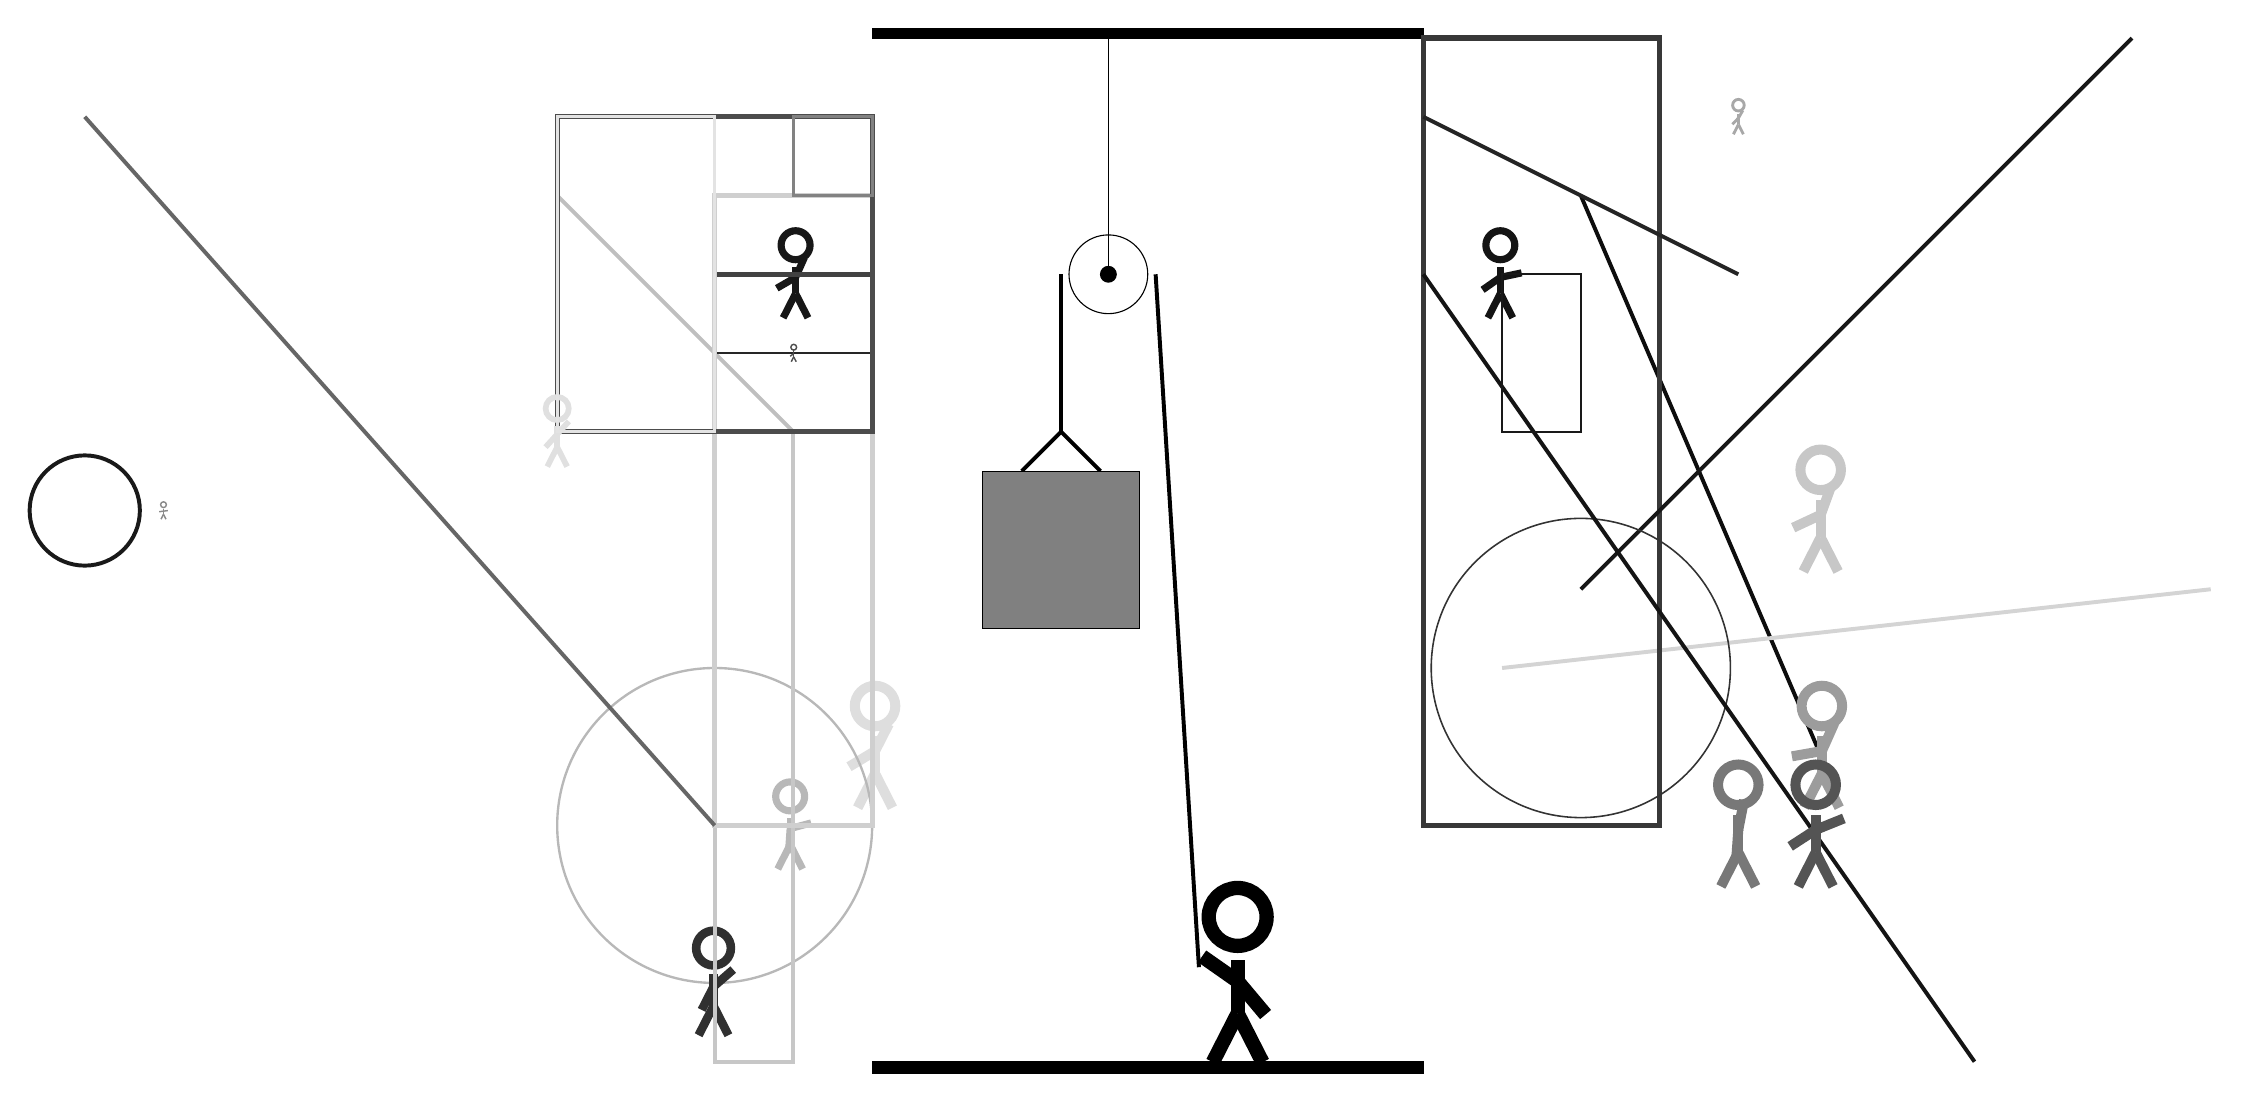
\begin{tikzpicture}
		%%%%% START %%%%%
		
		\draw[fill=black] (-2, 10) rectangle (5, 10.125);
		
		\draw (1, 7) circle (0.5);
		\draw[fill=black] (1, 7) circle (0.1);
		\draw (1, 10) -- (1, 7);
		
		\node[line width=0.7mm, color=black!22] at (10, 4) {\Strichmaxerl[7][25][70]};
		
		\draw[line width=0.5mm, color=black!95](10, 1) -- (7, 8);
		\draw[line width=0.5mm, color=black!17](6, 2) -- (15, 3);
		\draw [line width=0.5mm, color=black!90](-12, 4) circle (0.7);
		\node[line width=0.6mm, color=black!13] at (-2, 1) {\Strichmaxerl[7][31][63]};
		
		\draw [line width=0.3mm, color=black!28](-4, 0) circle (2.0);
		\draw[line width=0.5mm, color=black!25](-3, 5) -- (-6, 8);
		
		\node[line width=0.6mm, color=black!92] at (6, 7) {\Strichmaxerl[5][35][12]};
		\node[line width=0.6mm, color=black!91] at (-3, 7) {\Strichmaxerl[5][30][66]};
		
		\draw[line width=0.7mm, color=black!78] (5, 0) rectangle (8, 10);
		\draw[line width=0.6mm, color=black!74] (-4, 5) rectangle (-2, 7);
		\node[line width=0.3mm, color=black!28] at (-3, 0) {\Strichmaxerl[5][86][15]};
		\draw[line width=0.5mm, color=black!91](7, 3) -- (14, 10);
		
		\draw [line width=0.2mm, color=black!80](7, 2) circle (1.9);
		\node[line width=0.4mm, color=black!81] at (-4, -2) {\Strichmaxerl[6][63][41]};
		\node[line width=0.6mm, color=black!53] at (9, 0) {\Strichmaxerl[7][86][79]};
		
		\node[line width=0.7mm, color=black!34] at (9, 9) {\Strichmaxerl[2][46][60]};
		\node[line width=0.7mm, color=black!39] at (10, 1) {\Strichmaxerl[7][10][66]};
		\draw[line width=0.5mm, color=black!92](5, 7) -- (12, -3);
		\draw[line width=0.5mm, color=black!22] (-4, 5) rectangle (-3, -3);
		\draw[line width=0.3mm, color=black!85] (-4, 5) rectangle (-2, 6);
		
		\node[line width=0.4mm, color=black!67] at (10, 0) {\Strichmaxerl[7][33][22]};
		\draw[line width=0.3mm, color=black!90] (7, 5) rectangle (6, 7);
		\draw[line width=0.6mm, color=black!19] (-2, 0) rectangle (-4, 8);
		\node[line width=0.6mm, color=black!69] at (-3, 6) {\Strichmaxerl[1][36][90]};
		\draw[line width=0.6mm, color=black!70] (-2, 9) rectangle (-6, 5);
		\draw[line width=0.4mm, color=black!49] (-2, 9) rectangle (-3, 8);
		\draw[line width=0.5mm, color=black!60](-4, 0) -- (-12, 9);
		\node[line width=0.5mm, color=black!12] at (-6, 5) {\Strichmaxerl[4][48][48]};
		\draw[line width=0.5mm, color=black!86](5, 9) -- (9, 7);
		\draw[line width=0.4mm, color=black!11] (-4, 9) rectangle (-6, 5);
		
		\node[line width=0.7mm, color=black!46] at (-11, 4) {\Strichmaxerl[1][8][7]};
		
		\draw[line width=0.5mm] (-0.1, 4.5) -- (0.4, 5.0) -- (0.9, 4.5);
		\draw[fill=black!50] (-0.6, 4.5) rectangle (1.4, 2.5);
		
		\draw[line width=0.5mm] (0.4, 7) -- (0.4, 5.0);
		\centerarc[line width=0.5mm](1, 7)(0:180:0.6);
		\draw[line width=0.5mm](1.6, 7) -- (2.15, -1.8);
		
		\node at (2.6, -1.9) {\Strichmaxerl[10][-35][-50]};
		
		\draw[fill=black] (-2, -3) rectangle (5, -3.15);
		
		%%%%% END %%%%%
	\end{tikzpicture}
\end{document}